\subsection{Rangefinder Implementation}
With the data acquisition command tested and functioning properly, it needs to be connected to the ZedBoard. Since the rangefinder uses UART communication, there are a few reasonable options to create a UART controller on the ZedBoard.

\subsubsection{Rangefinder UART Options}
As the ZedBoard is such a powerful device, it has a few different options for controlling UART. A few of them are by controlling UART through linux, through a MicroBlaze soft-core processor, or through the Zynq-7000 Processing System. Running linux on the ZedBoard would use much of the board's valuable resources, and we would only be using a fraction of the capability provided by linux. The MicroBlaze soft-core processor would be a better alternative, but it runs in the programmable logic in the FPGA and is unnecessary when the ARM processor on the ZedBoard is unused \cite{microblaze}. Because of this, we decided to utilize the ARM processor on the ZedBoard by using the Zynq7 Processing System via Xilinx's Zynq-7000 Processing System Intellectual Property (IP) core.

\subsubsection{Zynq7 Processing System}
The ZedBoard SoC features a dual-core ARM Cortex-A9 MPCore processing system and Xilinx Programmable Logic. The Zynq7 Processing System IP core acts as a logic interface that integrates the Programmable Software (PS) with the Programmable Logic (PL), which allows access to both on-chip and external memory interfaces, to PL clocks, to many I/O peripherals, and even to extended I/O peripherals \cite{zynq7ps}. With all of this overwhelming functionality, the processing system is easy to customize, featuring a simple user interface (UI). The UI can be used to change the activated features. Figure \ref{zynq7ps_pic} below shows the processing system customization window.

\begin{figure}[H]
	\centerline{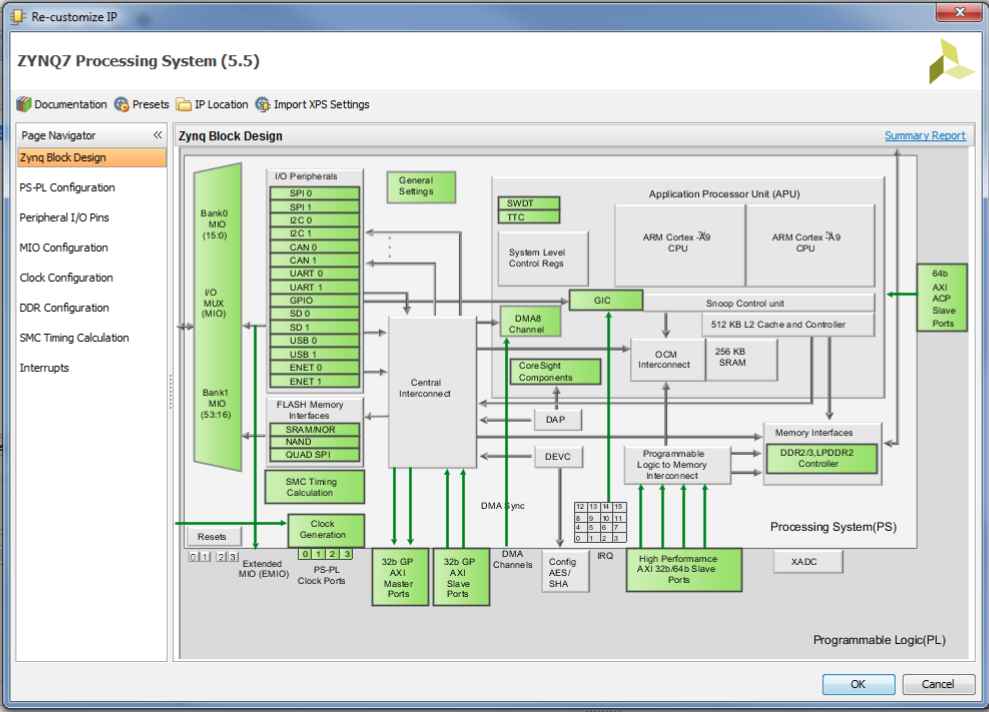
\includegraphics[width=1\textwidth]{zynq7ps.png}}
	\caption{Zynq7 Processing System Customization Window \cite{zynq7ps}}
	\label{zynq7ps_pic}
\end{figure}

In the figure above there are two options for UART shown: UART0 and UART1. explain difference between 0 and 1. say which one we chose. mio/emio. 

\subsubsection{PS-PL Communication}